%Exemplo de capitulo

\chapter{Redes Neurais Convolucionais}
\setcounter{figure}{100}

Rede neural artificial (ANN) é um modelo computacional inspirado na forma com
que o cérebro resolve problemas \cite{gilbert2000build}. Este modelo possui
unidades, denominadas neurônios, que possuem um valor que é calculado como uma
função do valor de outros neurônios.

\begin{figure}[!htb]
	\centering
	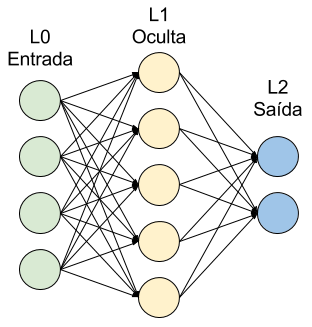
\includegraphics{ex_fcnn.png}
	\caption{Exemplo de rede neural totalmente conectada}
	\label{fig:ex_fcnn}
	(próprio autor).
\end{figure}

Alguns neurônios especiais, denominados “entradas” possuem um valor obtido de
fora do sistema. Estes são especiais porque são os únicos cujos valores não são
calculados. O valor de alguns dos neurônios de uma rede neural artificial podem
afetar sistemas externos à ela. Por isso são designados “saídas”. Neurônios que
não são de entrada ou de saída são chamados “ocultos”. A figura
\ref{fig:ex_fcnn} ilustra uma rede neural simples com os três tipos de
neurônios.

\section{Redes Neurais Não-Convolucionais}
As redes neurais artificiais são tipicamente organizadas em “camadas”, e a
escolha dos tipos de neurônio, juntamente com a forma com que os neurônios são
conectados, é denominada “topologia”. As redes são classificadas como
feedforward quando as conexões não formam ciclos ou recurrent quando formam. Se
uma camada está conectada a todos os neurônios da camada anterior diz-se que a
camada é totalmente conectada.
A definição da função de transferência do neurônio é uma parte importante da
topologia das redes neurais. Um tipo muito comum de neurônio é definido por:

\begin{equation} \label{eq:non-conv-layer}
	v=A \left( \left( \sum_n w_n i_n \right) + b \right)
\end{equation}

Onde v é o valor do neurônio, in é n-ésima entrada do neurônio, w é um vetor de
escalares denominado peso, e b é um escalar arbitrário, denominado bias. A é uma
função denominada função de ativação do neurônio. Essa função pode ser usada
para tornar o neurônio não-linear, como no caso da tangente hiperbólica. Os
pesos determinam a influência de cada entrada do neurônio.

A descrição de redes neurais com este tipo de neurônio e com topologia
totalmente conectada é especialmente conveniente. A camada de entrada é
representada por um vetor:

\begin{equation} \label{eq:l0}
	L0_{(4;1)}
\end{equation}

Para calcular a primeira camada intermediária é preciso aplicar
\ref{eq:non-conv-layer}. No caso de camadas totalmente conectadas cada
neurônio possui como entrada todos os
neurônios da camada anterior. Por este motivo $\sum_n w_n i_n$ pode ser
descrito como uma multiplicação de matrizes. O valor de todos os neurônios
da camada intermediária podem ser calculados com:

\begin{equation}
	L2_{(1;2)}=A_V \left( L1_{(1;2)} \cdot W2_{(5;2)} + B2_{(1;2)} \right)
\end{equation}

As matrizes $W$ e $B$ são os parâmetros que precisam ser aprendidos durante o
treinamento denominados parâmetros treináveis. O número de parâmetros de uma uma
rede neural é igual ao número de valores contidos em todas as matrizes de pesos
e bias. Quanto maior o número de parâmetros mais flexibilidade a rede neural
possui, porém mais lento é o treinamento. Se o número de parâmetros for
excessivo a rede neural perde a capacidade de generalizar e ocorre overfitting.

Como as dimensões da matriz de pesos são iguais ao número de entradas em uma
direção pelo número de saídas na outra direção, o número de parâmetros nessa
matriz é igual ao produto dos dois. Se uma camada convolucional tem 1000
entradas e 1000 saídas a matriz de pesos vai possuir 1.000.000 de parâmetros.

\section{Redes Neurais Convolucionais}
Redes neurais convolucionais operam sobre tensores, que são uma extensão de
vetores que admite um número arbitrário de dimensões. O motivo para isso é
permitir preservar a geometria da informação que está sendo processada. Uma
imagem bidimensional com dimensões $H$ e $W$ com C canais de cor vai ser
representada por um tensor de dimensões $H \times W \times C$. Uma imagem
tridimensional com 3
canais com profundidade $D$ é representada por um tensor
$D \times H \times W \times C$, e assim por
diante. Isso permite preservar o posicionamento relativo das informações durante
o processamento.

Caso a rede neural esteja operando sobre um tipo de informação que não possui o
conceito de “canal”, como séries temporais, é necessário artificialmente
criá-lo. Esse é o caso de séries temporais com “N” entradas, que serão
representadas por um tensor com dimensões $N\times1$. O motivo para isso é
uniformidade. O tensor de saída de uma camada convolucional inclui a dimensão
“canal”. Forçando tanto os tensores de entrada quanto de saída a incluírem um
canal o mesmo conceito de camada convolucional é aplicável em todas as camadas
com o mesmo número de dimensões.

A principal operação das redes neurais convolucionais é a cross-correlação:

\begin{equation}
	def: (f * g)[n] = \sum_{m=-\infty}^{\infty} f^*[m]g[m+n]
\end{equation}

Onde $f*$ é o complexo conjugado da função $f$. A cross-correlação é
equivalente à convolução de $f[n]$ com $g[-n]$. Uma camada de uma rede
neural que use qualquer uma das operações é denominada “convolucional”,
pois neste contexto as operações são intercambiáveis. A partir deste
ponto, apenas o termo “convolução” será usado.

Uma camada convolucional é definida pela a aplicação de um “kernel” sobre a
entrada dessa camada usando o operador convolução. O kernel, ou filtro é um
tensor a ser treinado. Se a entrada da camada convolucional tem dimensões
$D0 \times D1 \times D2 \times ... \times C$, onde C é o número de canais,
o filtro terá o mesmo número de dimensões, sendo que o tamanho de todas
as dimensões, exceto a última são
hiperparâmetros arbitrários. A última dimensão do filtro precisa ser igual ao
número de canais da imagem de entrada da camada convolucional, como ilustrado na
figura \ref{fig:ex_conv_2d}.


\begin{figure}[!htb]
	\centering
	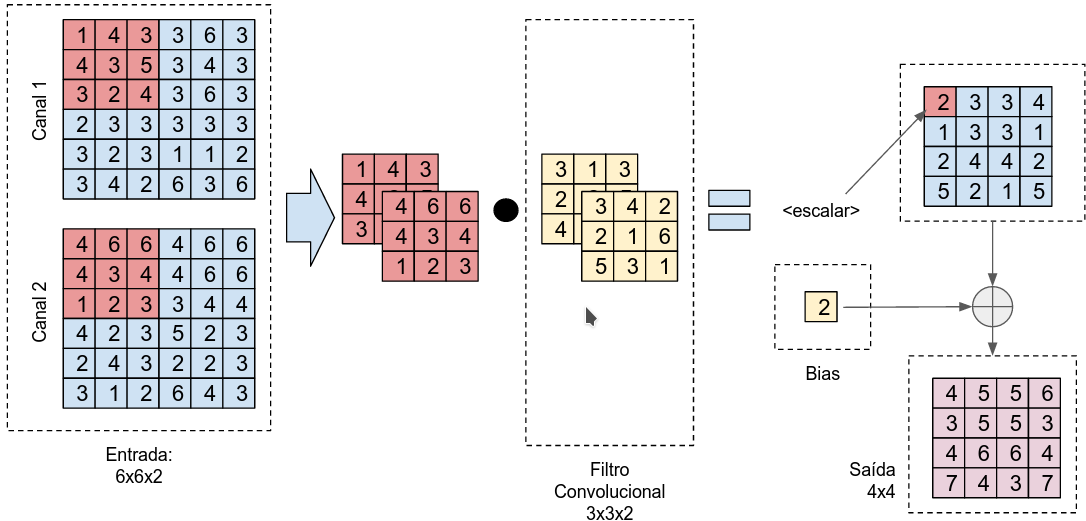
\includegraphics{ex_conv_2d.png}
	\caption{Exemplo de convolução 2D}
	\label{fig:ex_conv_2d}
	Exemplo da aplicação de uma única convolução sendo aplicada à uma imagem de
	entrada $6 \times 6 \times 2$. O tamanho da última dimensão do filtro e
	da entrada precisam ser iguais, no caso 2. As dimensões $3 \times 3$ do
	filtro foram escolhidas arbitrariamente. O símbolo do círculo na imagem
	representa um produto interno. A imagem de saída foi gerada deslocando
	a seleção de pixel a pixel (stride $1 \times 1$) até cobrir toda a
	imagem de entrada. Como as bordas não foram estendidas a imagem
	resultante é menor que a de entrada (próprio autor).
\end{figure}

Camadas convolucionais também usam o conceito de bias. Para isso o tensor
resultante da convolução é somado a um escalar. Este escalar é treinável e
permite, entre outras coisas, que a rede neural gere valores não-nulos mesmo que
a entrada seja nula.

\section{Bordas}
Na imagem \ref{fig:ex_conv_2d} o tamanho do tensor de saída foi reduzido
de 6 para 4. Pode ser
desejável fazer a saída ter o mesmo tamanho da entrada. Para isso é necessário
estender as bordas da imagem de entrada com zero, de forma a ser possível
aplicar o filtro inclusive nos pixels de borda, o que faria a saída ilustrada
nesta imagem ser $6 \times 6$.

A convolução só se encaixa corretamente na definição dada na equação X quando é
usada extensão de borda com zeros.

A opção de extensão de borda é um hiperparâmetro.

\section{Stride}
Ao se aplicar o filtro de convolução no tensor de entrada pode-se movê-lo de
posição a posição, até cobrir todos os locais válidos em cada direção, como
ilustrado na figura \ref{fig:ex_conv_2d}, ou pode-se desejar aplicar a cada
"$n_0$" pixels em uma direção, “$n_1$” pixels em outra direção, e assim por diante.
Esta opção é denominada \emph{stride}.

Quando uma camada convolucional possui como entrada um tensor de dimensões
$d1\times d2 \times ... \times dj \times C$ o stride é definido como sendo
um tensor unidimensional de tamanho j.
O stride $[1,2,1]$, por exemplo, indica que na primeira dimensão o
filtro será aplicado em todas as posições válidas, na segunda dimensão será
aplicado a cada 2 pixels e na terceira será aplicada novamente em todas as
posições válidas. Stride maior que 1 causa redução no tamanho do tensor de
saída.

Se um stride $2 \times 2$ fosse aplicado na convolução da figura
\ref{fig:ex_conv_2d} a imagem de saída seria $2 \times 2$.

\section{Profundidade do Filtro}
A figura \ref{fig:ex_conv_2d} mostrou um único filtro sendo aplicado ao
tensor de entrada. No
entanto, é possível aplicar um número arbitrário deles, sendo que cada filtro
produz um tensor de saída. Cada um destes filtros pode ser treinado para
reconhecer um feature diferente.

Se o tensor de entrada possui dimensões $d0 \times d1 \times ... \times C$
e deseja-se aplicar sobre este
tensor $N$ convoluções é possível representar isso com um único tensor
com dimensões
$N \times d0 \times d1 \times ... \times C$. Cada um dos filtros vai gerar
um tensor de saída, em um total de $N$. O
número de filtros é denominado “profundidade do filtro”. Todas as saídas podem
ser representadas em um único tensor com uma dimensão adicional. Usa-se a última
dimensão do tensor de saída para este fim. O motivo para isso é que cada uma
dessas saídas efetivamente se torna um “canal” de saída desta rede neural. No
exemplo da figura \ref{fig:ex_conv_2d}, se fossem aplicados 3 filtros a saída
seria um tensor $4 \times 4 \times 3$. Para isso o tensor que define o filtro
convolucional passaria a ser um
filtro de profundidade 3 descrito por um tensor de dimensões
$3 \times 4 \times 4 \times 2$.

\section{Processamento em Lotes}
Existem alguns cuidados especiais que devem ser tomados durante o treinamento de
redes neurais. Tomando o caso do treinamento supervisionado como exemplo, o
otimizador ajusta os parâmetros treináveis da rede neural para tentar reduzir o
erro. Para verificar se a alteração teve sucesso a rede neural é alimentada com
dados etiquetados, e o valor de saída da rede neural é comparado com os dados
esperados. É conveniente fornecer vários exemplos etiquetados, não apenas um, e
usar a média do erro para alimentar o otimizador. A idéia é que o valor passado
seja o mais representativo possível.

O número de imagens fornecidas é denominado “tamanho do batch”. Se uma rede
neural trabalha com dados de dimensões $d0 \times d1 \times ... \times C$
pode-se agrupar “B” exemplos em
um único tensor, com dimensões $B \times d0 \times d1 \times ... \times C$.
As camadas convolucionais tratam cada
uma das imagens separadamente, conforme já foi descrito, e emite na sua saída um
único tensor que também usa uma dimensão adicional para agrupar as diferentes
imagens.

O valor de B não é um hiperparâmetro, mas sim um parâmetro de treinamento.

\section{Pooling}
Após a aplicação de uma camada convolucional pode-se aplicar uma camada de
\emph{pooling}, que é uma forma de subamostragem. A figura
\ref{fig:ex_maxpool} ilustra uma operação de maxpool, que é um tipo de
pooling.

\begin{figure}[!htb]
	\centering
	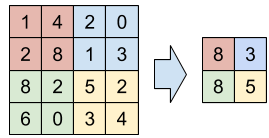
\includegraphics{ex_maxpool.png}
	\caption{Exemplo de \emph{maxpool} $2 \times 2$}
	\label{fig:ex_maxpool}
	Ilustração de uma operação maxpool $2 \times 2$ aplicado usando stride
	$2 \times 2$. O filtro move de dois em dois pixels e possui
	tamanho 2 em cada dimensão (próprio autor).
\end{figure}

Esta operação possui como parâmetros o tamanho do filtro, o stride e a opção de
borda. A operação a ser aplicada no filtro pode ser $max$ ou $avg$ (média),
que definem respectivamente os filtros \emph{maxpool} e \emph{avgpool}.

Como as operações de pooling são normalmente feitas com stride maior que 1 elas
acabam reduzindo consideravelmente o tamanho do tensor de saída. No caso de um
maxpool $2 \times 2$, por exemplo, o tensor resultante vai ter 25\% do
número de valores do tensor de entrada.

\section{ReLu}
Assim como em redes neurais totalmente conectadas, pode-se aplicar uma função de
ativação para aumentar a não-linearidade. Pode-se usar as funções tangente
hiperbólica, sigmóide ou outras tipicamente usadas em redes neurais
não-convolucionais. No entanto a função ReLu, ou linear retificada, resulta em
treinamento substancialmente mais rápido enquanto mantém a capacidade de
generalização da rede neural treinada. A função ReLu é definida por:


\begin{equation}
	ReLu(x) = max(0,x)
\end{equation}

\section{Últimas Camadas}
Após as camadas convolucionais terem sido aplicadas é necessário usar um
classificador, mecanismo de regressão ou outro sistema que gere o tipo de saída
desejada para a rede neural. Uma das possíveis formas de realizar esta função é
usar uma ou duas camadas totalmente conectadas, como ilustrado na figura
\ref{fig:ex_cnn}. No exemplo a função de ativação da penúltima camada é
ReLu e a última camada é linear.

\section{Rede Neural Convolucional Completa}
Para alguns casos simples pode-se construir uma rede neural convolucional
conectando-se uma camada convolucional à uma maxpool e uma ReLu. Este conjunto
pode ser repetido algumas vezes até que o número de saídas da camada
convolucional seja baixo o suficiente para que seja passado por duas camadas
totalmente conectadas. Se houver interesse em não reduzir o tamanho total do
tensor pode-se omitir a camada maxpool. Um exemplo dessa topologia é a figura
\ref{fig:ex_cnn}.

A topologia da rede neural e o conjunto de todos os hiperparâmetros definem o
número de parâmetros treináveis que a rede neural vai possuir e quantas
operações são necessárias para aplicar a rede neural em um (ou um lote de)
amostras. Uma rede neural mais larga, com um maior número de filtros por
camadas, possui a capacidade de aprender mais features. Redes neurais mais
profundas possuem capacidade de abstração maior, sendo capazes de inferir a
partir dos dados de entrada conceitos mais complexos.

\begin{figure}[!htb]
	\centering
	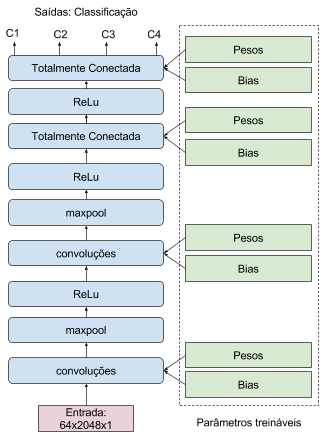
\includegraphics{ex_cnn.png}
	\caption{Exemplo de rede neural convolucional completa}
	\label{fig:ex_cnn}
	Esta rede neural possui nove camadas para
	classificação de séries temporais em uma de 4 classes. Destaca-se os
	parâmetros treináveis (próprio autor).
\end{figure}

\section{Uso em Processamento de Imagens}
O uso de redes neurais convolucionais é uma alternativa a diversos métodos já
existentes de detecção de objetos em imagens. Aqui serão mostradas algumas das
alternativas usuais, para que sejam contrastadas com a classificação baseada em
redes neurais convolucionais.

\subsection{Redes Neurais Não-Convolucionais}
Quando uma imagem vai ser processada por uma rede não-convolucional ela precisa
ser convertida para a forma plana, em um vetor com dimensões
$(1; H \cdot W \cdot C)$.

O uso de camadas totalmente conectadas é proibitivo para classificação de
imagens desta maneira. Se uma rede neural for usada para processar imagens de 1
megapixel, ou 720x1280, e a primeira camada possuir um número de neurônios igual
ao número de neurônios da camada de entrada, a matriz de pesos teria
$(720 \cdot 1280 \cdot 3)^2 \approx 7.6 \cdot 10^{12}$ parâmetros. Se for
representado por números ponto-flutuante de 32 bits isso ocuparia mais de
30 TiB. O mesmo processo em uma imagem 480px por 640px geraria quase 850
bilhões de parâmetros só na matriz de pesos.

Outras topologias mais esparsas podem ser construídas, mas este tipo de rede
neural possui outros problemas que as tornam inviáveis para processamento direto
de imagens. Um exemplo é o fato delas não serem invariantes ao deslocamento. Se
a rede neural aprende a reconhecer um feature em um local da imagem não vai
conseguir reaproveitar essa capacidade em outras posições. Portanto teria que
aprender a mesma feature em cada possível posição onde ela possa aparecer, e
fazer isso para todas as features.

Como a primeira operação feita foi converter a imagem para um formato “plano”, a
geometria da imagem foi destruída. Não é mais possível determinar quando dois
pixels estão próximos, e essa é uma informação muito importante sobre a imagem.

\subsection{Redes Neurais Convolucionais em Imagens}
\subsection{Uso de Cores}
\subsection{Reconhecimento de Objetos}
\subsection{Localização de Objetos}

